\documentclass{standalone}
\usepackage{tikz}
\usetikzlibrary{arrows,decorations.markings}

\begin{document}

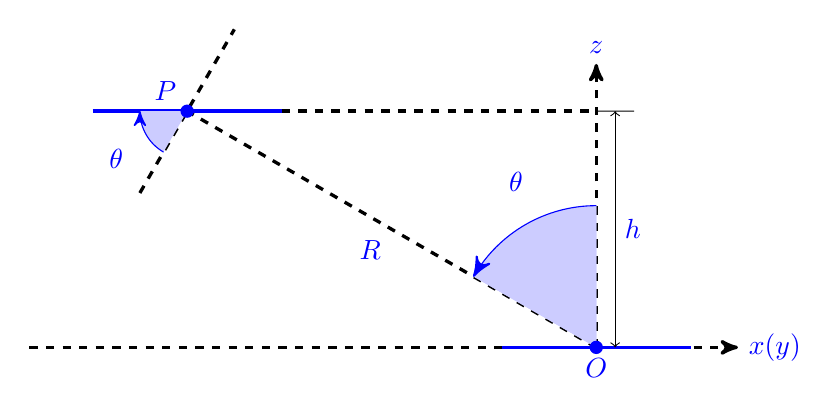
\begin{tikzpicture}[
  scale=6,
  axis/.style={dashed, very thick, ->, >=stealth'},
  important line/.style={very thick, color=blue},
  dashed line/.style={dashed, very thick},
  every node/.style={color=blue}
  ]
  \draw[axis] (-1.2,0)  -- (.3,0) node(xline)[right]
      {$x(y)$};
  \draw[axis] (0,0) -- (0,.6) node(yline)[above] {$z$};
  \draw[dashed line] (0,0) coordinate (O) node [below] {$O$} -- ({-.5*sqrt(3)/2}, {.5/2}) node [below left] {$R$} -- ({-.5*sqrt(3)}, .5) coordinate (P) node [above left] {$P$};
  \draw[important line] (-.2,0) -- (.2,0);
  \draw[important line] ({-.5*sqrt(3)-.2},.5) -- ({-.5*sqrt(3)+.2},.5);
  \draw[dashed line] ({-.5*sqrt(3)-.1},{.5-.1*sqrt(3)}) coordinate (P') -- ({-.5*sqrt(3)+.1},{.5+.1*sqrt(3)});
  \draw[dashed line] ({-.5*sqrt(3)+.2},.5) -- (0,.5) coordinate (h);
  \draw (h) -- (.08,.5);
  \draw[<->] (.04,0) -- (.04,.25) node [right] {$h$} -- (.04,.5);

  \fill[fill=blue!20!white] (90:3mm) arc (90:150:3mm) -- (0,0) -- cycle; % Following https://tex.stackexchange.com/a/62140
  \fill[fill=blue!20!white] (90:3mm) arc (90:150:3mm) -- (0,0) -- cycle;
  % \fill[fill=blue!20!white] ({-.5*sqrt(3)}-.05, .5-.05*sqrt(3)) arc (90:150:3mm) -- ({-.5*sqrt(3)}, .5) -- cycle;
  \fill[fill=blue!20!white] (P) -- ({-.5*sqrt(3)-.05},{.5-.05*sqrt(3)}) coordinate (P'') arc (240:180:.1) -- ({-.5*sqrt(3)}, .5);

  \node at (-.17,.35) {$\theta$};
  \node at ({-.5*sqrt(3)-.15}, .5-.1) {$\theta$};

  \draw[blue, decoration={markings,mark=at position 1 with
  {\arrow[scale=2,>=stealth']{>}}},postaction={decorate}] (90:3mm) arc (90:150:3mm);
  \draw[blue, decoration={markings,mark=at position 1 with
  {\arrow[scale=1.5,>=stealth']{>}}},postaction={decorate}] (P'') arc (240:180:.1);

  \fill[blue] (P) circle (.4pt);
  \fill[blue] (O) circle (.4pt);
\end{tikzpicture}

\end{document}